\documentclass[conference]{IEEEtran}
\IEEEoverridecommandlockouts
% The preceding line is only needed to identify funding in the first footnote. If that is unneeded, please comment it out.
% \usepackage{cite}
% Enables Portuguese Brasil
% \usepackage[portuguese]{babel}
%encoding
\usepackage[numbers]{natbib}
% Enables code listing
\usepackage{listings}
%--------------------------------------
\usepackage[T1]{fontenc}
\usepackage[utf8]{inputenc}
%--------------------------------------
%Enables the use of greek letter without a math context
\usepackage{textgreek}
%--------------------------------------
%Enables hiperlinks
\usepackage[hidelinks]{hyperref}
%--------------------------------------

\usepackage{amsmath,amssymb,amsfonts}
\usepackage{algorithmic}
\usepackage{graphicx}
\usepackage{textcomp}
\usepackage{xcolor}

\usepackage{color, colortbl}

% The code style
\usepackage{color}
\definecolor{codegreen}{rgb}{0,0.6,0}
\definecolor{codegray}{rgb}{0.5,0.5,0.5}
\definecolor{codepurple}{rgb}{0.58,0,0.82}
\definecolor{backcolour}{rgb}{0.95,0.95,0.92}

\lstdefinestyle{mystyle}{
	backgroundcolor=\color{backcolour},   
	commentstyle=\color{codegreen},
	keywordstyle=\color{magenta},
	numberstyle=\tiny\color{codegray},
	stringstyle=\color{codepurple},
	basicstyle=\footnotesize,
	breakatwhitespace=false,         
	breaklines=true,                 
	captionpos=b,                    
	keepspaces=true,                 
	numbers=left,                    
	numbersep=2pt,                  
	showspaces=false,                
	showstringspaces=false,
	showtabs=false,                  
	tabsize=2
}
\lstset{style=mystyle}
%---------------------------------------

\def\BibTeX{{\rm B\kern-.05em{\sc i\kern-.025em b}\kern-.08em
		T\kern-.1667em\lower.7ex\hbox{E}\kern-.125emX}}

\title{Introdução à Computação Quântica}

\institute{Universidade Estadual Paulista Júlio de Mesquita Filho}

\author{André Furlan - ensismoebius@gmail.com}

\logo{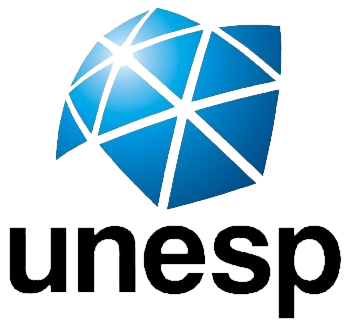
\includegraphics[height=1cm]{unesp.png}}
\date{\the\year}

\begin{document}
	
	\frame{\titlepage}
	
	\begin{frame}{Introdução}
		\begin{itemize}
			\item A mecânica quântica surgiu no século XX, juntamente com os computadores clássicos.
			\item A computação quântica tem recebido atenção significativa devido ao seu potencial para resolver problemas complexos de forma mais eficiente do que os computadores clássicos.
			\item A computação quântica utiliza os princípios da mecânica quântica para realizar cálculos usando bits quânticos ou qubits.
		\end{itemize}
	\end{frame}
	
	\begin{frame}{Estados Quânticos}
		\begin{itemize}
			\item Os estados quânticos são representações matemáticas que fornecem informações sobre as propriedades de um sistema físico, como a posição ou o momento de uma partícula.
			\item Os estados quânticos são descritos usando vetores de estado, que são frequentemente representados usando a notação de Dirac "ket" (por exemplo, $|\psi\rangle$).
			\item Ao contrário dos bits clássicos, que podem representar apenas 0 ou 1, os estados quânticos podem existir em uma superposição, onde eles representam simultaneamente vários estados possíveis.
		\end{itemize}
	\end{frame}
	
	\begin{frame}{Espaço Vetorial Complexo}
		\begin{itemize}
			\item Os estados quânticos são representados usando espaços vetoriais complexos.
			\item Um espaço vetorial complexo é uma estrutura matemática que segue regras específicas, incluindo comutatividade e associatividade, permitindo a combinação de vetores.
			\item Os vetores de base dentro do espaço vetorial representam os estados possíveis do sistema quântico, e as combinações lineares desses vetores de base representam estados quânticos arbitrários.
		\end{itemize}
	\end{frame}
	
	\begin{frame}{Notação de Dirac}
		\begin{itemize}
			\item A notação de "BraKet" de Dirac, desenvolvida pelo físico Paul Dirac, é uma notação comum usada na mecânica quântica.
			\item A notação "ket" ($|\psi\rangle$) representa o estado de uma partícula dentro do espaço vetorial.
			\item A notação "bra" ($\langle\psi|$) representa o transposto conjugado do vetor ket.
			\item O produto interno de um bra e um ket fornece a amplitude de probabilidade para um determinado estado.
		\end{itemize}
	\end{frame}
	
	\begin{frame}{Amplitude de Probabilidade}
		\begin{itemize}
			\item As amplitudes de probabilidade são números complexos que descrevem a probabilidade de ocorrência de um estado quântico específico.
			\item As amplitudes de probabilidade são calculadas usando o produto interno de um bra e um ket.
			\item As amplitudes de probabilidade são normalizadas para garantir que a soma das probabilidades de todos os estados possíveis seja igual a 1.
		\end{itemize}
	\end{frame}
	
	\begin{frame}{Operadores Lineares}
		\begin{itemize}
			\item Os operadores lineares são ferramentas matemáticas usadas para descrever transformações em espaços vetoriais.
			\item Na mecânica quântica, os operadores lineares representam observáveis físicos, como posição, momento e energia.
			\item Os operadores lineares podem ser aplicados a vetores de estado para obter novos vetores de estado resultantes da transformação.
		\end{itemize}
	\end{frame}
	
	\begin{frame}{Operadores Lineares (cont.)}
		\begin{itemize}
			\item Exemplos de operadores lineares comumente usados na mecânica quântica incluem o operador de posição, operador de momento e operador de energia.
			\item Esses operadores têm propriedades específicas, como hermiticidade e comutatividade, que são importantes na mecânica quântica.
		\end{itemize}
	\end{frame}
	
	\begin{frame}{Portas Quânticas}
		\begin{itemize}
			\item Portas quânticas são análogas aos circuitos lógicos em computadores clássicos.
			\item Elas são operadores lineares que agem em qubits individuais ou em múltiplos qubits.
			\item As portas quânticas permitem a transformação dos estados quânticos, possibilitando várias operações computacionais.
			\item Algumas portas quânticas conhecidas incluem a porta Hadamard, porta Pauli-X e a porta CNOT.
		\end{itemize}
	\end{frame}
	
	\begin{frame}{Portas Quânticas (cont.)}
		\begin{itemize}
			\item Porta Hadamard: Ela cria uma superposição de estados em um qubit. É representada pela seguinte matriz:
			\[
			H = \frac{1}{\sqrt{2}}\begin{bmatrix}
				1 & 1 \\
				1 & -1 \\
			\end{bmatrix}
			\]
			\item Porta Pauli-X: Conhecida como porta NOT quântica, ela inverte o estado de um qubit. É representada pela seguinte matriz:
			\[
			X = \begin{bmatrix}
				0 & 1 \\
				1 & 0 \\
			\end{bmatrix}
			\]
			\item Porta CNOT: A porta Controlled NOT opera em dois qubits, onde um atua como controle e o outro como alvo. É representada pela seguinte matriz:
			\[
			CNOT = \begin{bmatrix}
				1 & 0 & 0 & 0 \\
				0 & 1 & 0 & 0 \\
				0 & 0 & 0 & 1 \\
				0 & 0 & 1 & 0 \\
			\end{bmatrix}
			\]
		\end{itemize}
	\end{frame}
	
	\begin{frame}{Conclusão}
		\begin{itemize}
			\item A computação quântica é um campo promissor que utiliza os princípios da mecânica quântica para realizar cálculos mais eficientes.
			\item Os estados quânticos, espaços vetoriais complexos, operadores lineares e portas quânticas são conceitos fundamentais na computação quântica.
			\item As portas quânticas permitem a realização de operações computacionais, e exemplos conhecidos incluem a porta Hadamard, porta Pauli-X e porta CNOT.
			\item A compreensão desses conceitos é essencial para explorar o potencial da computação quântica e suas aplicações futuras.
		\end{itemize}
	\end{frame}
	
	\begin{frame}[allowframebreaks]
		\frametitle{Referências}
		\bibliography{bibliography.bib}
	\end{frame}
	
\end{document}